%\begin{figure}[!h] % option !h pour dire que l'image sera à cet endroit
%	\centering
%	\includegraphics[scale=0.5]{../images/siege_interlog.jpg}
%	\caption{Siège social, Interlog Services à Orléans}
%	\label{Siege interlog}
%\end{figure}

\mysection{\interlog}

	\begin{photo}[!h]
		\centering
		\includegraphics[scale=0.5]{./images/siege_interlog.jpg}
		\caption{Siège social, \interlog à Orléans}
	\end{photo}

	\mysubsection{Présentation de l'entreprise}
		Anciennement \textit{ipseurope}, \interlog a été créé en 1999. Il s'agit de la première société à proposer sur le continent européen des audits de factures de transport.\\

		La société intervient au coeur de la \og Supply-Chain\fg \footnote{chaîne logistique}  et propose des prestations permettant des gains non négligeables. Les clients viennent de tous les secteurs d'activités (luxe, agroalimentaire, automobile \ldots).  \\

		Les équipes d'\interlog sont spécialisées dans la logistique et interviennent quotidiennement dans la gestion des opérations des clients. Elles interviennent sur:
		\begin{itemize}
			\item l'audit des factures transport,
			\item la gestion intégrée d’expéditions,
			\item l'organisation personnalisée du transport,
			\item le pilotage de plans de transport,
			\item l'approvisionnements mutualisés,
			\item le suivi et traçabilité des livraisons.
		\end{itemize}	
		
		\interlog  a su se développer à l'étranger. Elle est présente sur la France, l'Inde, les États-Unis et le Mexique.\\
		
		La société a pour but de réduire les coûts de transport des entreprises qui font appel a ses services.

    

    
    
    
   
